It is unlikely to have a model perform as one expects the first time. There are
therefore a few techniques for optimizing the performance. It should be noted
that much of the discussion here and in Section \ref{sec:valid} focuses on
the diagnostics aspect rather than the validation aspect of these techniques.
In practice, these are used for both purposes, but in this work the formal
comparison of model performance will be used, introduced and demonstrated in
Sections \ref{sec:invcompare} and \ref{sec:algcompare}, respectively. 

However, the increase in performance from over-optimization could be linked to
the training set performance and might not generalize outside of the specific
type of input data used.  A workaround for this scenario is to obtain more data
for the set or to obtain a completely different data set altogether. 

\subsubsection{Training Set Size}

The first diagnostic plot for optimizing the model performance is called a
\textit{learning curve}, which provides information about the bias-variance
tradeoff with respect to the data set size. More specifically, learning curves
compare the training and cross-validation errors to the size of the training
set (i.e., number of instances in the training set). This is done by randomly
selecting a percentage of the the training set, inputting that into a
statistical learner, and tabulating the error of the learned model. 

Typically, a learning curve will look somewhat like one of the three examples
in Figure \ref{fig:learning}.  A learning curve tests the model for high bias
or high variance, which can correspond to an undefit or overfit model,
respectively. 

\begin{figure}[!hp]
  \centering
  \begin{subfigure}[h]{0.65\linewidth}
    \centering
    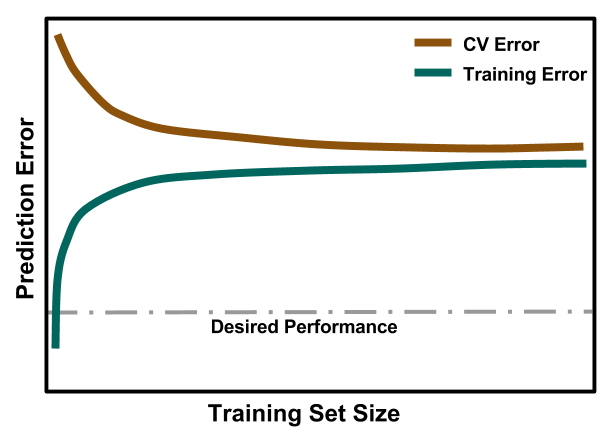
\includegraphics[width=\linewidth]{./chapters/litrev/LearningCurve-bias.png}
    \caption{High bias}
    \label{fig:bias}
  \end{subfigure}
  \begin{subfigure}[h]{0.65\linewidth}
    \centering
    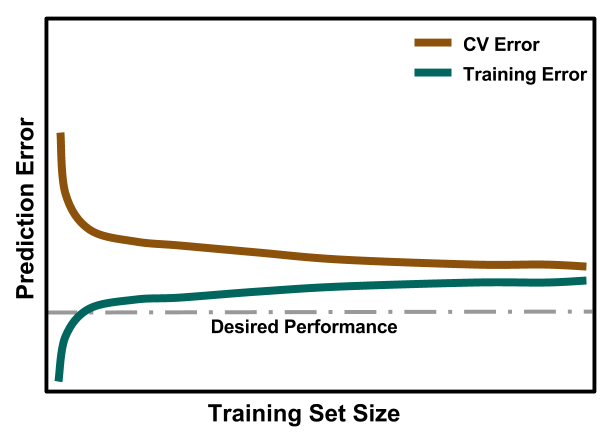
\includegraphics[width=\linewidth]{./chapters/litrev/LearningCurve-ideal.png}
    \caption{Ideal}
    \label{fig:ideal}
  \end{subfigure}
  \begin{subfigure}[h]{0.65\linewidth}
    \centering
    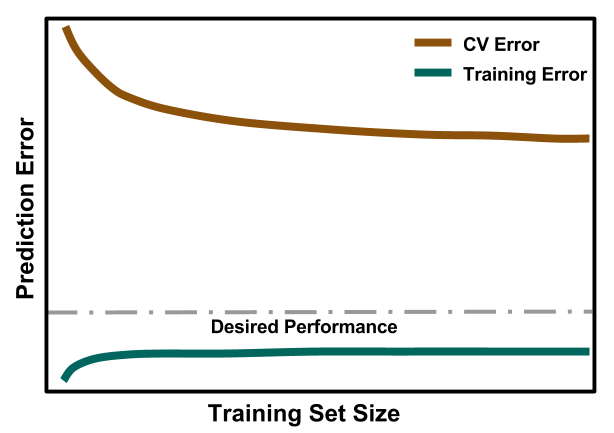
\includegraphics[width=\linewidth]{./chapters/litrev/LearningCurve-variance.png}
    \caption{High variance}
    \label{fig:variance}
  \end{subfigure}
  \caption{Learning curves for three training scenarios}
  \label{fig:learning}
\end{figure}
\todo{add reference}

Figure \ref{fig:bias} suggests underfitting because the model is missing
important features in the data. It is characterized by a small gap between the
curves but high overall errors. The cross-validation error remains consistently
high and the training error increases drastically with increasing data, since
it is not generalizing well. 

Figure \ref{fig:variance} suggests overfitting because the model has too much
sensitivity to variations in the data. It is characterized by a very large gap
between the curves. It has an extremely low training error, as it has taken
into account every detail of the training set, but a high cross-validation
error because it cannot generalize beyond the testing set. 

Figure \ref{fig:ideal} is an example of a more ideal model fit. It is
characterized by a small gap between the two errors, and they are at a
reasonable level with respect to the desired performance.  The training error
should increase with respect to the training set size due to a larger amount of
bias (preventing overfitting). But the cross-validation error should decrease
quickly with respect to the training set size due to being close to the minimum
of the bias-variance tradeoff. 

\subsubsection{Model Complexity}

After ensuring the appropriate training set size is selected, the models must
be further optimized using \textit{validation curves}.  These provide
information on the bias-variance tradeoff with respect to model complexity. Two
main factors affecting model complexity can cause the model to be under- or
overfit to the data: number of features in the data set and algorithm
parameters that vary the regularization.

\begin{figure}[!htb]
  \centering
  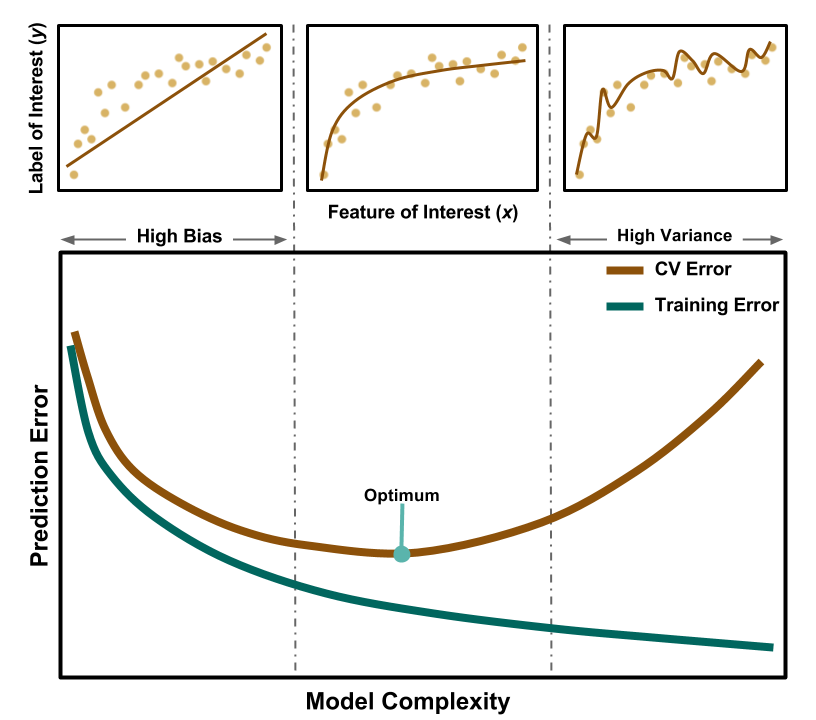
\includegraphics[width=1.05\linewidth]{./chapters/litrev/ValidationCurve.png}
  \caption{Validation curve showing examples of different fittings}
  \label{fig:validation}
\end{figure}

Figure \ref{fig:validation} adapted from Ref. \cite{elements_stats} shows the
optimum as the minimum of the cross-validation error curve. There is some gap
between it and the training error, much larger than the left side of the plot
and much smaller than the right.  The plot above is a visualization of a
decently fit model.  The left region is marked by both errors being quite high,
and above is an  illustration of how an underfit plot (high bias) could provide
high errors. The right region shows the training error being quite low but the
cross-validation error being high. The diagram above shows that it is obvious
how the training error would be negligible, but generalizing beyond that
probably will not yield accurate results. 

In practice, plotting learning and validation curves can be iterative. But as
previously mentioned, too many optimizations will result in a poorly performing
model when exposed to data outside of the training set.

\subsubsection{Comparison of Methods}
\label{sec:invcompare}

In addition to evaluating a single learned model, it may be beneficial to
compare models. This can be done using Bayesian inference as discussed in
Section \ref{sec:inverse} \cite{inverse_theory}.  Equations \ref{eq:bayes} and
\ref{eq:bayes_words} show that there are three values to obtain to calculate a
probability of a parameter estimated from a machine-learned model being
correct: the prior probability, the likelihood, and the marginal likelihood.
The marginal likelihood is only needed for absolute posterior probability
calculations; it does not affect the relative probabilities, which are all that
is needed for model comparison.

The prior probabilities are obtained by a large set of forward problems, e.g.,
a database of spent fuel recipes and parameters. In this study, this is
provided by the training data set that is comprised of simulated \gls{SNF}
recipes. The likelihoods are obtained in differing ways from the model space.
One method is expert-elicited values. Another is a predicted model from some
established theory or previously known relationship, e.g., empirical relations
between isotopic ratios and certain reactor parameters or a direct calculation
of the reactor parameters \cite{inverse_theory}. In this study, it is obtained
from the estimated model parameters from a given statistical model. 

